\documentclass[]{article}

\usepackage[]{geometry}
\geometry{
  top=1in,            % <-- you want to adjust this
  inner=1in,
  outer=1in,
  bottom=1in,
  headheight=3ex,       % <-- and this
  headsep=2ex,          % <-- and this
}
\usepackage[T1]{fontenc}
\usepackage{cmbright}
\usepackage{mathtools}
\usepackage{algorithmic}
\usepackage{fancyhdr}
\usepackage{amssymb}
\usepackage{multicol}
\usepackage{parskip}
\usepackage{titling}
\usepackage{fancyvrb}
\pretitle{\begin{flushleft}\LARGE\sffamily}
\posttitle{\par\end{flushleft}\vskip 0.5em}
\preauthor{\begin{flushleft}}
\postauthor{\par\end{flushleft}}
\predate{\begin{flushleft}\scshape}
\postdate{\par\end{flushleft}}
\setlength{\droptitle}{-20pt}
\setlength{\headheight}{15.2pt}
\pagestyle{fancy}

\setcounter{secnumdepth}{1}

\fancyhf{}
\renewcommand{\headrulewidth}{0pt} % remove line at top
\lhead{\fancyplain{}{CS 4320 A1}}
\rhead{\fancyplain{}{Justin Cheng \emph{jc882}}}
\rfoot{\fancyplain{}{\thepage}}

\begin{document}

\title{CS 4780 Assignment 3}
\author{Justin Cheng and Sunling Selena Yang}
\date{\today}
\maketitle

\hrule
\vskip 1em

\section{Perceptron and SVM}
\subsection{a.}
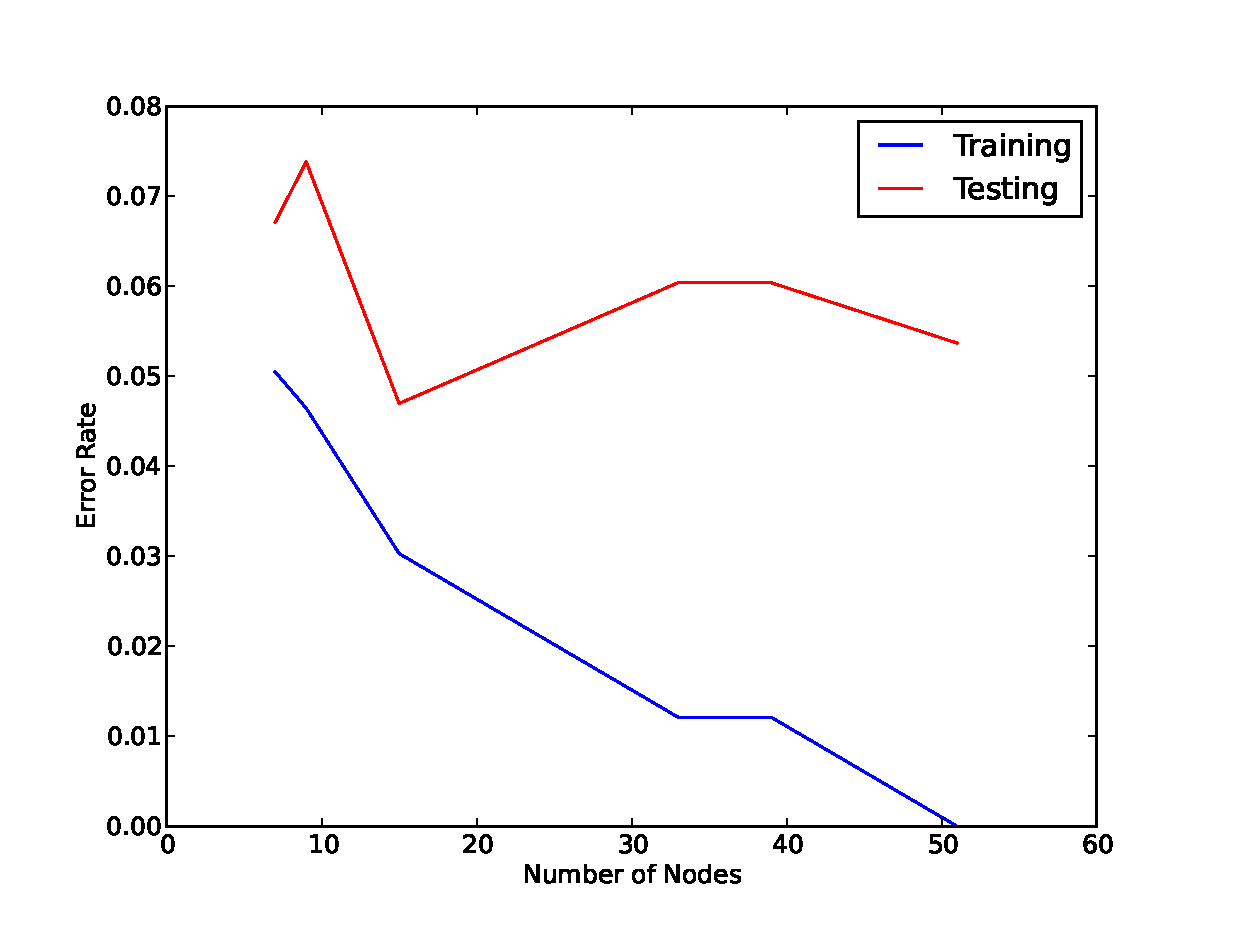
\includegraphics[scale=0.5]{data/images/part_a.eps}

The training error decreases dramatically after the first few iterations, although it is not strictly decreasing. However, after the 15th iteration the training error is 0, meaning that a separating hyperplane was learnt.

The validation error fluctuates wildly for the first few iterations, but then stabilizes at about 0.217.

This does appear to confirm the fact that the Perceptron algorithm converges after a finite number of iterations.

Prefer a lower learning rate for improved accuracy, though over a longer number of iterations. If the learning rate is too high, over-correction is likely to occur and you might end up oscillating around the true separating hyperplane.

We should not use the dual algorithm, since it stores needless information and requires us to keep the whole training set in memory, even when we perform predictions. If we don't care about the $\alpha$s, we can simply use the primal algorithm to update $w_k$ incrementally. (TODO how about accuracy?)

\subsection{b.}
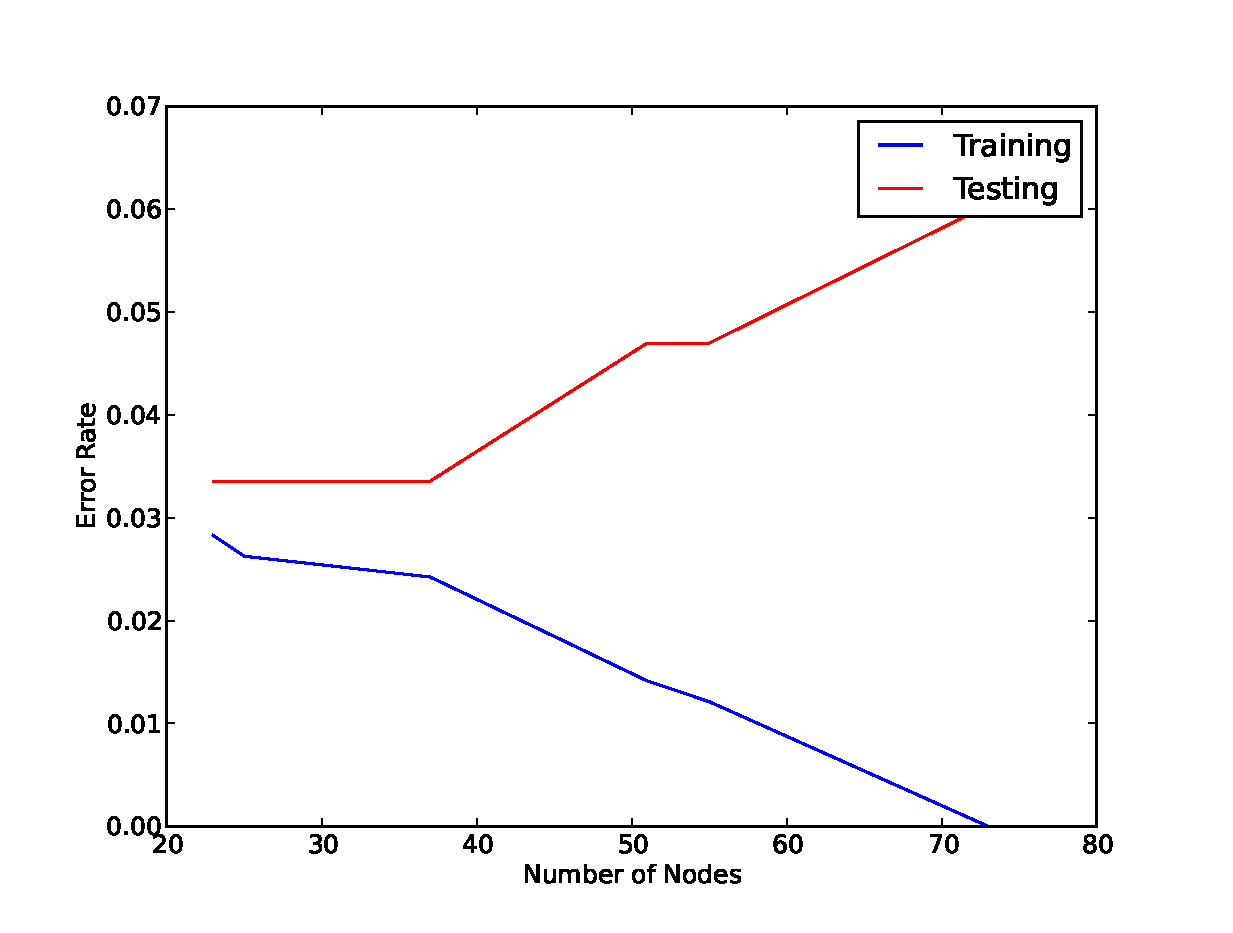
\includegraphics[scale=0.5]{data/images/part_b.eps}

The smallest validation error rate is achieved at $C = 8$. (TODO compare to (a)).

The training error rate goes to 0 as C increases, but the validation error steadily decreases to a minimum at $C=8$, and increases after that. (TODO Why?)

\subsection{c.}
(TODO Perceptron)

Using $SVM_{light}$ with $C=8$, the training error in all cases is 0.009, and the validation error in all cases is 0.205. 

\end{document}